%% An Introduction to LaTeX Thesis Template of Wuhan University
%%
%% Created by WHUTUG

% 用来设置附录中代码的样式



\documentclass[type=master,oneside]{whu-thesis}
\whusetup
{
  info               =
    {
      title          = {图像有损压缩Matlab仿真及性能测试},
      title*         = {}, 
      student-number = {2021202120085},
      school         = {电子信息学院},
      author         = {陈子昂,朱鹤然,卢意帆},
      author*        = {Chen Ziang, Zhu Heran, Lu Yifan},
      subject        = {学科},
      major          = {电子信息学院},
      advisor        = {茹国宝},
      direction      = {信息与通信工程},
      % date           = {2021/5},
      keywords       = {关键词 1 , 关键词 2 , 关键词 3 , 关键词 4 , 一个非常非常,非常非常长——的关键词 5},
      keywords*      = {key word 1 , key word 2 , key word 3 , key word 4 , {and a very very, very very long key word---the key word 5}},
    },
  style              =
    {
      graphics-path  = {{figures/}{data/}},
    },
  element            =
    {
      abstract       = {pages/abstract},
      % bibliography   = {ref/refs},
      appendix       = {pages/appendix}
    }
}
% 
\usepackage{ctex}
\usepackage{listings}  % 排代码用的宏包
\usepackage{color}
\definecolor{codegreen}{rgb}{0,0.6,0}
\definecolor{codegray}{rgb}{0.5,0.5,0.5}
\definecolor{codepurple}{rgb}{0.58,0,0.82}
\definecolor{backcolour}{rgb}{0.95,0.95,0.92}
\usepackage{fontspec}
\setmonofont{Consolas}
\lstset{
    basicstyle        =   \ttfamily\footnotesize,
    keywordstyle      =   \color{codepurple}\bfseries,% 关键字颜色
    identifierstyle   =   \color{blue},
    % showstringspaces  =   false, % 不显示字符串内的空格
    backgroundcolor   =   \color[rgb]{0.98,0.98,0.98},% 背景颜色
    numbers           =   left, % 显示行号 left right none
    xleftmargin       =   3em, %整体距左侧边线的距离为2em
    xrightmargin      =   1em,
    % 中文代码
    commentstyle      =   \ttfamily\color{codegreen},                % 设置代码注释的格式
    breaklines,% 自动换行,建议不要写太长的行
    showstringspaces  =   false,
    breakatwhitespace =   true,
    % escapeinside      = ``,%逃逸字符(1左面的键),用于显示中文例如在代码中`中文...`
    tabsize           = 2,
    extendedchars     = false %解决代码跨页时,章节标题,页眉等汉字不显示的问题
}



\usepackage{hyperref}
\hypersetup{
	colorlinks=true,
	linkcolor=cyan,
	filecolor=blue,      
	urlcolor=red,
	citecolor=green,
}

\begin{document}
%%----------- 主体部分 ----------- %%
\chapter{图像有损压缩技术的背景}

\section{图像压缩概述}

原始的数字图像数据可以占用相当大的存储空间,在计算机的存储、传输、处理等环节将产生很大的计算处理负担,因此图像数据的压缩就显得非常重要了。

例如一张尺寸为3840\times2180的原始图像,如果每个像素使用32bit(RGBA)来表示,那么存储这一张图像需要占用的空间为 3840\times2180\times4=33484800Byte≈31.9MB。相应的,如果拍摄1 分钟 30 帧(fps)的4k视频,那么需要的存储空间将会达到3840\times2180\times4\times30\times60 ≈ 56.1GB。由此看来,对于图像视频,尤其是视频的数据压缩就显得尤为重要了。

图像数据是用来表示图像信息的,不同的方法表示相同的图像信息会使用不同的数据量,不同的方法中,必然会有一些会产生不必要的重复或者无用信息,重复的信息属于不相干信息,无用的信息属于冗余信息。图像压缩编码的主要目的,就是通过删除冗余的或者是不相干的信息,以尽可能小的存储、尽可能低的码率来传输数字图像数据。

信息时代带来了“信息爆炸”,使数据量大增,因此,无论传输或存储都需要对数据进行有效的压缩。在遥感技术中,各种航天探测器采用压缩编码技术,将获取的巨大信息送回地面。


\section{图像压缩的基本原理}

图像数据之所以能被压缩,就是因为图像数据中存在着冗余部分。
图像数据的冗余主要表现为4种:
\begin{itemize}
    \item \textbf{空间冗余}。一幅图像表面上各像素点之间往往存在着空间连贯性,相邻像素之前也存在相关性,由此产生的空间冗余;
    \item \textbf{时间冗余}。视频的相邻帧往往包含相同的背景和移动物体,相邻帧之间存在相关性,由此产生的时间冗余;
    \item \textbf{频谱冗余}。不同彩色平面或频谱带之间存在相关,由此产生的频谱冗余;
    \item \textbf{视觉冗余}。人类的视觉系统由于受生理特性的限制,对于图像场的注意是非均匀的,人对细微的颜色差异感觉不明显。
\end{itemize}

\section{图像压缩的分类}
根据压缩后的图像是否能完全恢复,可以将图像压缩技术分为无损压缩和有损压缩两类。
\subsection{图像的无损压缩}

利用无损压缩方法消除或减少的各种形式的冗余可以重新插入到数据中,因此,无损压缩是可逆过程,也称无失真压缩。

为了消除或减少数据中的冗余度,常常要用信源的统计特性或建立信源的统计模型,因此许多实用的无损压缩技术均可归结为统计编码方法。

统计编码方法中常用的有 Huffman 编码、算术编码、RLE(Run Length Encoding)编码等。 此外统计编码技术在各种有损压缩 方法中也有广泛的应用。

\subsection{图像的有损压缩}

有损压缩法压缩了熵,信息量会减少,而损失的信息量不能再恢复,因此有损压缩是不可逆过程。 有损压缩主要有两大类:特征 提取和量化方法。 特征提取的编码方法如模型基编码、分形编码等。 量化是有损压缩最基本的形式,其优点是可以得到比无损压缩 高得多的压缩比。 有损压缩只能用于允许一定程度失真的情况,比如对图像、声音、视频等数据的压缩。
无损压缩和有损压缩结合形成了混合编码技术,它融合了各种不同的压缩编码技术,很多国际标准都是采用混合编码技术,如 JPEG,MPEG 等标准。 利用混合编码对自然景物的灰度图像进行压缩一般可压缩几倍到十几倍,而对于自然景物的彩色图像压缩比 将达到几十甚至上百倍。

\section{图像压缩的发展现状}

早在1948年,当电视信号数字化之后,图像压缩的研究就逐渐展开了,1952年,哈夫曼提出了“最小冗余代码构造方法”\cite{最小冗余代码构造方法},1968年,Elisa发展了香农和费诺的编码方法\cite{elias1955coding},1976年,算术编码的方法\cite{rissanen1976generalized}被提出,1982年算术编码预测模型结合。20世纪80年代,由于神经网络的应用逐步广泛,1987年,就提出了人工神经网络预测编码,1994年,JPEG\cite{wallace1992jpeg}标准正式成为国际标准,在7年后的2001年,JPEG2000\cite{rabbani2002jpeg2000}正式确立。近年来,随着深度学习技术的不断发展深入,越来越多的深度学习技术被应用在了图像编码算法上,例如2016年Balle等人提出的卷积神经网络CNN图像编码框架\cite{balle2016end},2017年Rippel和Bourde发表了基于生成对抗网络GAN的图像编码器\cite{rippel2017real},同年,Google的研究人员提出了循环神经网络RNN的图像编码器\cite{toderici2017full}。

%% An Introduction to LaTeX Thesis Template of Wuhan University
%%
%% Created by WHUTUG

% 用来设置附录中代码的样式



\documentclass[type=master,oneside]{whu-thesis}
\whusetup
{
  info               =
    {
      title          = {图像有损压缩Matlab仿真及性能测试},
      title*         = {}, 
      student-number = {2021202120085},
      school         = {电子信息学院},
      author         = {陈子昂,朱鹤然,卢意帆},
      author*        = {Chen Ziang, Zhu Heran, Lu Yifan},
      subject        = {学科},
      major          = {电子信息学院},
      advisor        = {茹国宝},
      direction      = {信息与通信工程},
      % date           = {2021/5},
      keywords       = {关键词 1 , 关键词 2 , 关键词 3 , 关键词 4 , 一个非常非常,非常非常长——的关键词 5},
      keywords*      = {key word 1 , key word 2 , key word 3 , key word 4 , {and a very very, very very long key word---the key word 5}},
    },
  style              =
    {
      graphics-path  = {{figures/}{data/}},
    },
  element            =
    {
      abstract       = {pages/abstract},
      % bibliography   = {ref/refs},
      appendix       = {pages/appendix}
    }
}
% 
\usepackage{ctex}
\usepackage{listings}  % 排代码用的宏包
\usepackage{color}
\definecolor{codegreen}{rgb}{0,0.6,0}
\definecolor{codegray}{rgb}{0.5,0.5,0.5}
\definecolor{codepurple}{rgb}{0.58,0,0.82}
\definecolor{backcolour}{rgb}{0.95,0.95,0.92}
\usepackage{fontspec}
\setmonofont{Consolas}
\lstset{
    basicstyle        =   \ttfamily\footnotesize,
    keywordstyle      =   \color{codepurple}\bfseries,% 关键字颜色
    identifierstyle   =   \color{blue},
    commentstyle      =   \color{codegreen}% 注释颜色
    % showstringspaces  =   false, % 不显示字符串内的空格
    breaklines        =   true,   % 自动换行,建议不要写太长的行
    backgroundcolor   =   \color[rgb]{0.98,0.98,0.98},% 背景颜色
    numbers           =   left, % 显示行号 left right none
    xleftmargin       =   3em, %整体距左侧边线的距离为2em
    xrightmargin      =   1em,
    % 中文代码
    breaklines        = true,
    breakatwhitespace = true,
    escapeinside      = ``,%逃逸字符(1左面的键),用于显示中文例如在代码中`中文...`
    tabsize           = 4,
    extendedchars     = false %解决代码跨页时,章节标题,页眉等汉字不显示的问题  
}



\usepackage{hyperref}
\hypersetup{
	colorlinks=true,
	linkcolor=cyan,
	filecolor=blue,      
	urlcolor=red,
	citecolor=green,
}

\begin{document}
%%----------- 主体部分 ----------- %%
\chapter{图像有损压缩技术的背景}

\section{图像压缩概述}

原始的数字图像数据可以占用相当大的存储空间,在计算机的存储、传输、处理等环节将产生很大的计算处理负担,因此图像数据的压缩就显得非常重要了。

例如一张尺寸为3840\times2180的原始图像,如果每个像素使用32bit(RGBA)来表示,那么存储这一张图像需要占用的空间为 3840\times2180\times4=33484800Byte≈31.9MB。相应的,如果拍摄1 分钟 30 帧(fps)的4k视频,那么需要的存储空间将会达到3840\times2180\times4\times30\times60 ≈ 56.1GB。由此看来,对于图像视频,尤其是视频的数据压缩就显得尤为重要了。

图像数据是用来表示图像信息的,不同的方法表示相同的图像信息会使用不同的数据量,不同的方法中,必然会有一些会产生不必要的重复或者无用信息,重复的信息属于不相干信息,无用的信息属于冗余信息。图像压缩编码的主要目的,就是通过删除冗余的或者是不相干的信息,以尽可能小的存储、尽可能低的码率来传输数字图像数据。

信息时代带来了“信息爆炸”,使数据量大增,因此,无论传输或存储都需要对数据进行有效的压缩。在遥感技术中,各种航天探测器采用压缩编码技术,将获取的巨大信息送回地面。


\section{图像压缩的基本原理}

图像数据之所以能被压缩,就是因为图像数据中存在着冗余部分。
图像数据的冗余主要表现为4种:
\begin{itemize}
    \item \textbf{空间冗余}。一幅图像表面上各像素点之间往往存在着空间连贯性,相邻像素之前也存在相关性,由此产生的空间冗余;
    \item \textbf{时间冗余}。视频的相邻帧往往包含相同的背景和移动物体,相邻帧之间存在相关性,由此产生的时间冗余;
    \item \textbf{频谱冗余}。不同彩色平面或频谱带之间存在相关,由此产生的频谱冗余;
    \item \textbf{视觉冗余}。人类的视觉系统由于受生理特性的限制,对于图像场的注意是非均匀的,人对细微的颜色差异感觉不明显。
\end{itemize}

\section{图像压缩的分类}
根据压缩后的图像是否能完全恢复,可以将图像压缩技术分为无损压缩和有损压缩两类。
\subsection{图像的无损压缩}

利用无损压缩方法消除或减少的各种形式的冗余可以重新插入到数据中,因此,无损压缩是可逆过程,也称无失真压缩。

为了消除或减少数据中的冗余度,常常要用信源的统计特性或建立信源的统计模型,因此许多实用的无损压缩技术均可归结为统计编码方法。

统计编码方法中常用的有 Huffman 编码、算术编码、RLE(Run Length Encoding)编码等。 此外统计编码技术在各种有损压缩 方法中也有广泛的应用。

\subsection{图像的有损压缩}

有损压缩法压缩了熵,信息量会减少,而损失的信息量不能再恢复,因此有损压缩是不可逆过程。 有损压缩主要有两大类:特征 提取和量化方法。 特征提取的编码方法如模型基编码、分形编码等。 量化是有损压缩最基本的形式,其优点是可以得到比无损压缩 高得多的压缩比。 有损压缩只能用于允许一定程度失真的情况,比如对图像、声音、视频等数据的压缩。
无损压缩和有损压缩结合形成了混合编码技术,它融合了各种不同的压缩编码技术,很多国际标准都是采用混合编码技术,如 JPEG,MPEG 等标准。 利用混合编码对自然景物的灰度图像进行压缩一般可压缩几倍到十几倍,而对于自然景物的彩色图像压缩比 将达到几十甚至上百倍。

\section{图像压缩的发展现状}

早在1948年,当电视信号数字化之后,图像压缩的研究就逐渐展开了,1952年,哈夫曼提出了“最小冗余代码构造方法”\cite{最小冗余代码构造方法},1968年,Elisa发展了香农和费诺的编码方法\cite{elias1955coding},1976年,算术编码的方法\cite{rissanen1976generalized}被提出,1982年算术编码预测模型结合。20世纪80年代,由于神经网络的应用逐步广泛,1987年,就提出了人工神经网络预测编码,1994年,JPEG\cite{wallace1992jpeg}标准正式成为国际标准,在7年后的2001年,JPEG2000\cite{rabbani2002jpeg2000}正式确立。近年来,随着深度学习技术的不断发展深入,越来越多的深度学习技术被应用在了图像编码算法上,例如2016年Balle等人提出的卷积神经网络CNN图像编码框架\cite{balle2016end},2017年Rippel和Bourde发表了基于生成对抗网络GAN的图像编码器\cite{rippel2017real},同年,Google的研究人员提出了循环神经网络RNN的图像编码器\cite{toderici2017full}。

%% An Introduction to LaTeX Thesis Template of Wuhan University
%%
%% Created by WHUTUG

% 用来设置附录中代码的样式



\documentclass[type=master,oneside]{whu-thesis}
\whusetup
{
  info               =
    {
      title          = {图像有损压缩Matlab仿真及性能测试},
      title*         = {}, 
      student-number = {2021202120085},
      school         = {电子信息学院},
      author         = {陈子昂,朱鹤然,卢意帆},
      author*        = {Chen Ziang, Zhu Heran, Lu Yifan},
      subject        = {学科},
      major          = {电子信息学院},
      advisor        = {茹国宝},
      direction      = {信息与通信工程},
      % date           = {2021/5},
      keywords       = {关键词 1 , 关键词 2 , 关键词 3 , 关键词 4 , 一个非常非常,非常非常长——的关键词 5},
      keywords*      = {key word 1 , key word 2 , key word 3 , key word 4 , {and a very very, very very long key word---the key word 5}},
    },
  style              =
    {
      graphics-path  = {{figures/}{data/}},
    },
  element            =
    {
      abstract       = {pages/abstract},
      % bibliography   = {ref/refs},
      appendix       = {pages/appendix}
    }
}
% 
\usepackage{ctex}
\usepackage{listings}  % 排代码用的宏包
\usepackage{color}
\definecolor{codegreen}{rgb}{0,0.6,0}
\definecolor{codegray}{rgb}{0.5,0.5,0.5}
\definecolor{codepurple}{rgb}{0.58,0,0.82}
\definecolor{backcolour}{rgb}{0.95,0.95,0.92}
\usepackage{fontspec}
\setmonofont{Consolas}
\lstset{
    basicstyle        =   \ttfamily\footnotesize,
    keywordstyle      =   \color{codepurple}\bfseries,% 关键字颜色
    identifierstyle   =   \color{blue},
    commentstyle      =   \color{codegreen}% 注释颜色
    % showstringspaces  =   false, % 不显示字符串内的空格
    breaklines        =   true,   % 自动换行,建议不要写太长的行
    backgroundcolor   =   \color[rgb]{0.98,0.98,0.98},% 背景颜色
    numbers           =   left, % 显示行号 left right none
    xleftmargin       =   3em, %整体距左侧边线的距离为2em
    xrightmargin      =   1em,
    % 中文代码
    breaklines        = true,
    breakatwhitespace = true,
    escapeinside      = ``,%逃逸字符(1左面的键),用于显示中文例如在代码中`中文...`
    tabsize           = 4,
    extendedchars     = false %解决代码跨页时,章节标题,页眉等汉字不显示的问题  
}



\usepackage{hyperref}
\hypersetup{
	colorlinks=true,
	linkcolor=cyan,
	filecolor=blue,      
	urlcolor=red,
	citecolor=green,
}

\begin{document}
%%----------- 主体部分 ----------- %%
\chapter{图像有损压缩技术的背景}

\section{图像压缩概述}

原始的数字图像数据可以占用相当大的存储空间,在计算机的存储、传输、处理等环节将产生很大的计算处理负担,因此图像数据的压缩就显得非常重要了。

例如一张尺寸为3840\times2180的原始图像,如果每个像素使用32bit(RGBA)来表示,那么存储这一张图像需要占用的空间为 3840\times2180\times4=33484800Byte≈31.9MB。相应的,如果拍摄1 分钟 30 帧(fps)的4k视频,那么需要的存储空间将会达到3840\times2180\times4\times30\times60 ≈ 56.1GB。由此看来,对于图像视频,尤其是视频的数据压缩就显得尤为重要了。

图像数据是用来表示图像信息的,不同的方法表示相同的图像信息会使用不同的数据量,不同的方法中,必然会有一些会产生不必要的重复或者无用信息,重复的信息属于不相干信息,无用的信息属于冗余信息。图像压缩编码的主要目的,就是通过删除冗余的或者是不相干的信息,以尽可能小的存储、尽可能低的码率来传输数字图像数据。

信息时代带来了“信息爆炸”,使数据量大增,因此,无论传输或存储都需要对数据进行有效的压缩。在遥感技术中,各种航天探测器采用压缩编码技术,将获取的巨大信息送回地面。


\section{图像压缩的基本原理}

图像数据之所以能被压缩,就是因为图像数据中存在着冗余部分。
图像数据的冗余主要表现为4种:
\begin{itemize}
    \item \textbf{空间冗余}。一幅图像表面上各像素点之间往往存在着空间连贯性,相邻像素之前也存在相关性,由此产生的空间冗余;
    \item \textbf{时间冗余}。视频的相邻帧往往包含相同的背景和移动物体,相邻帧之间存在相关性,由此产生的时间冗余;
    \item \textbf{频谱冗余}。不同彩色平面或频谱带之间存在相关,由此产生的频谱冗余;
    \item \textbf{视觉冗余}。人类的视觉系统由于受生理特性的限制,对于图像场的注意是非均匀的,人对细微的颜色差异感觉不明显。
\end{itemize}

\section{图像压缩的分类}
根据压缩后的图像是否能完全恢复,可以将图像压缩技术分为无损压缩和有损压缩两类。
\subsection{图像的无损压缩}

利用无损压缩方法消除或减少的各种形式的冗余可以重新插入到数据中,因此,无损压缩是可逆过程,也称无失真压缩。

为了消除或减少数据中的冗余度,常常要用信源的统计特性或建立信源的统计模型,因此许多实用的无损压缩技术均可归结为统计编码方法。

统计编码方法中常用的有 Huffman 编码、算术编码、RLE(Run Length Encoding)编码等。 此外统计编码技术在各种有损压缩 方法中也有广泛的应用。

\subsection{图像的有损压缩}

有损压缩法压缩了熵,信息量会减少,而损失的信息量不能再恢复,因此有损压缩是不可逆过程。 有损压缩主要有两大类:特征 提取和量化方法。 特征提取的编码方法如模型基编码、分形编码等。 量化是有损压缩最基本的形式,其优点是可以得到比无损压缩 高得多的压缩比。 有损压缩只能用于允许一定程度失真的情况,比如对图像、声音、视频等数据的压缩。
无损压缩和有损压缩结合形成了混合编码技术,它融合了各种不同的压缩编码技术,很多国际标准都是采用混合编码技术,如 JPEG,MPEG 等标准。 利用混合编码对自然景物的灰度图像进行压缩一般可压缩几倍到十几倍,而对于自然景物的彩色图像压缩比 将达到几十甚至上百倍。

\section{图像压缩的发展现状}

早在1948年,当电视信号数字化之后,图像压缩的研究就逐渐展开了,1952年,哈夫曼提出了“最小冗余代码构造方法”\cite{最小冗余代码构造方法},1968年,Elisa发展了香农和费诺的编码方法\cite{elias1955coding},1976年,算术编码的方法\cite{rissanen1976generalized}被提出,1982年算术编码预测模型结合。20世纪80年代,由于神经网络的应用逐步广泛,1987年,就提出了人工神经网络预测编码,1994年,JPEG\cite{wallace1992jpeg}标准正式成为国际标准,在7年后的2001年,JPEG2000\cite{rabbani2002jpeg2000}正式确立。近年来,随着深度学习技术的不断发展深入,越来越多的深度学习技术被应用在了图像编码算法上,例如2016年Balle等人提出的卷积神经网络CNN图像编码框架\cite{balle2016end},2017年Rippel和Bourde发表了基于生成对抗网络GAN的图像编码器\cite{rippel2017real},同年,Google的研究人员提出了循环神经网络RNN的图像编码器\cite{toderici2017full}。

%% An Introduction to LaTeX Thesis Template of Wuhan University
%%
%% Created by WHUTUG

% 用来设置附录中代码的样式



\documentclass[type=master,oneside]{whu-thesis}
\whusetup
{
  info               =
    {
      title          = {图像有损压缩Matlab仿真及性能测试},
      title*         = {}, 
      student-number = {2021202120085},
      school         = {电子信息学院},
      author         = {陈子昂,朱鹤然,卢意帆},
      author*        = {Chen Ziang, Zhu Heran, Lu Yifan},
      subject        = {学科},
      major          = {电子信息学院},
      advisor        = {茹国宝},
      direction      = {信息与通信工程},
      % date           = {2021/5},
      keywords       = {关键词 1 , 关键词 2 , 关键词 3 , 关键词 4 , 一个非常非常,非常非常长——的关键词 5},
      keywords*      = {key word 1 , key word 2 , key word 3 , key word 4 , {and a very very, very very long key word---the key word 5}},
    },
  style              =
    {
      graphics-path  = {{figures/}{data/}},
    },
  element            =
    {
      abstract       = {pages/abstract},
      % bibliography   = {ref/refs},
      appendix       = {pages/appendix}
    }
}
% 
\usepackage{ctex}
\usepackage{listings}  % 排代码用的宏包
\usepackage{color}
\definecolor{codegreen}{rgb}{0,0.6,0}
\definecolor{codegray}{rgb}{0.5,0.5,0.5}
\definecolor{codepurple}{rgb}{0.58,0,0.82}
\definecolor{backcolour}{rgb}{0.95,0.95,0.92}
\usepackage{fontspec}
\setmonofont{Consolas}
\lstset{
    basicstyle        =   \ttfamily\footnotesize,
    keywordstyle      =   \color{codepurple}\bfseries,% 关键字颜色
    identifierstyle   =   \color{blue},
    commentstyle      =   \color{codegreen}% 注释颜色
    % showstringspaces  =   false, % 不显示字符串内的空格
    breaklines        =   true,   % 自动换行,建议不要写太长的行
    backgroundcolor   =   \color[rgb]{0.98,0.98,0.98},% 背景颜色
    numbers           =   left, % 显示行号 left right none
    xleftmargin       =   3em, %整体距左侧边线的距离为2em
    xrightmargin      =   1em,
    % 中文代码
    breaklines        = true,
    breakatwhitespace = true,
    escapeinside      = ``,%逃逸字符(1左面的键),用于显示中文例如在代码中`中文...`
    tabsize           = 4,
    extendedchars     = false %解决代码跨页时,章节标题,页眉等汉字不显示的问题  
}



\usepackage{hyperref}
\hypersetup{
	colorlinks=true,
	linkcolor=cyan,
	filecolor=blue,      
	urlcolor=red,
	citecolor=green,
}

\begin{document}
%%----------- 主体部分 ----------- %%
\include{pages/background}
\include{pages/jpeg}
\include{pages/evaluation}
\end{document}
\chapter{图像有损压缩实验结果}

\section{实验结果的定性分析}
\begin{figure}
    \centering
    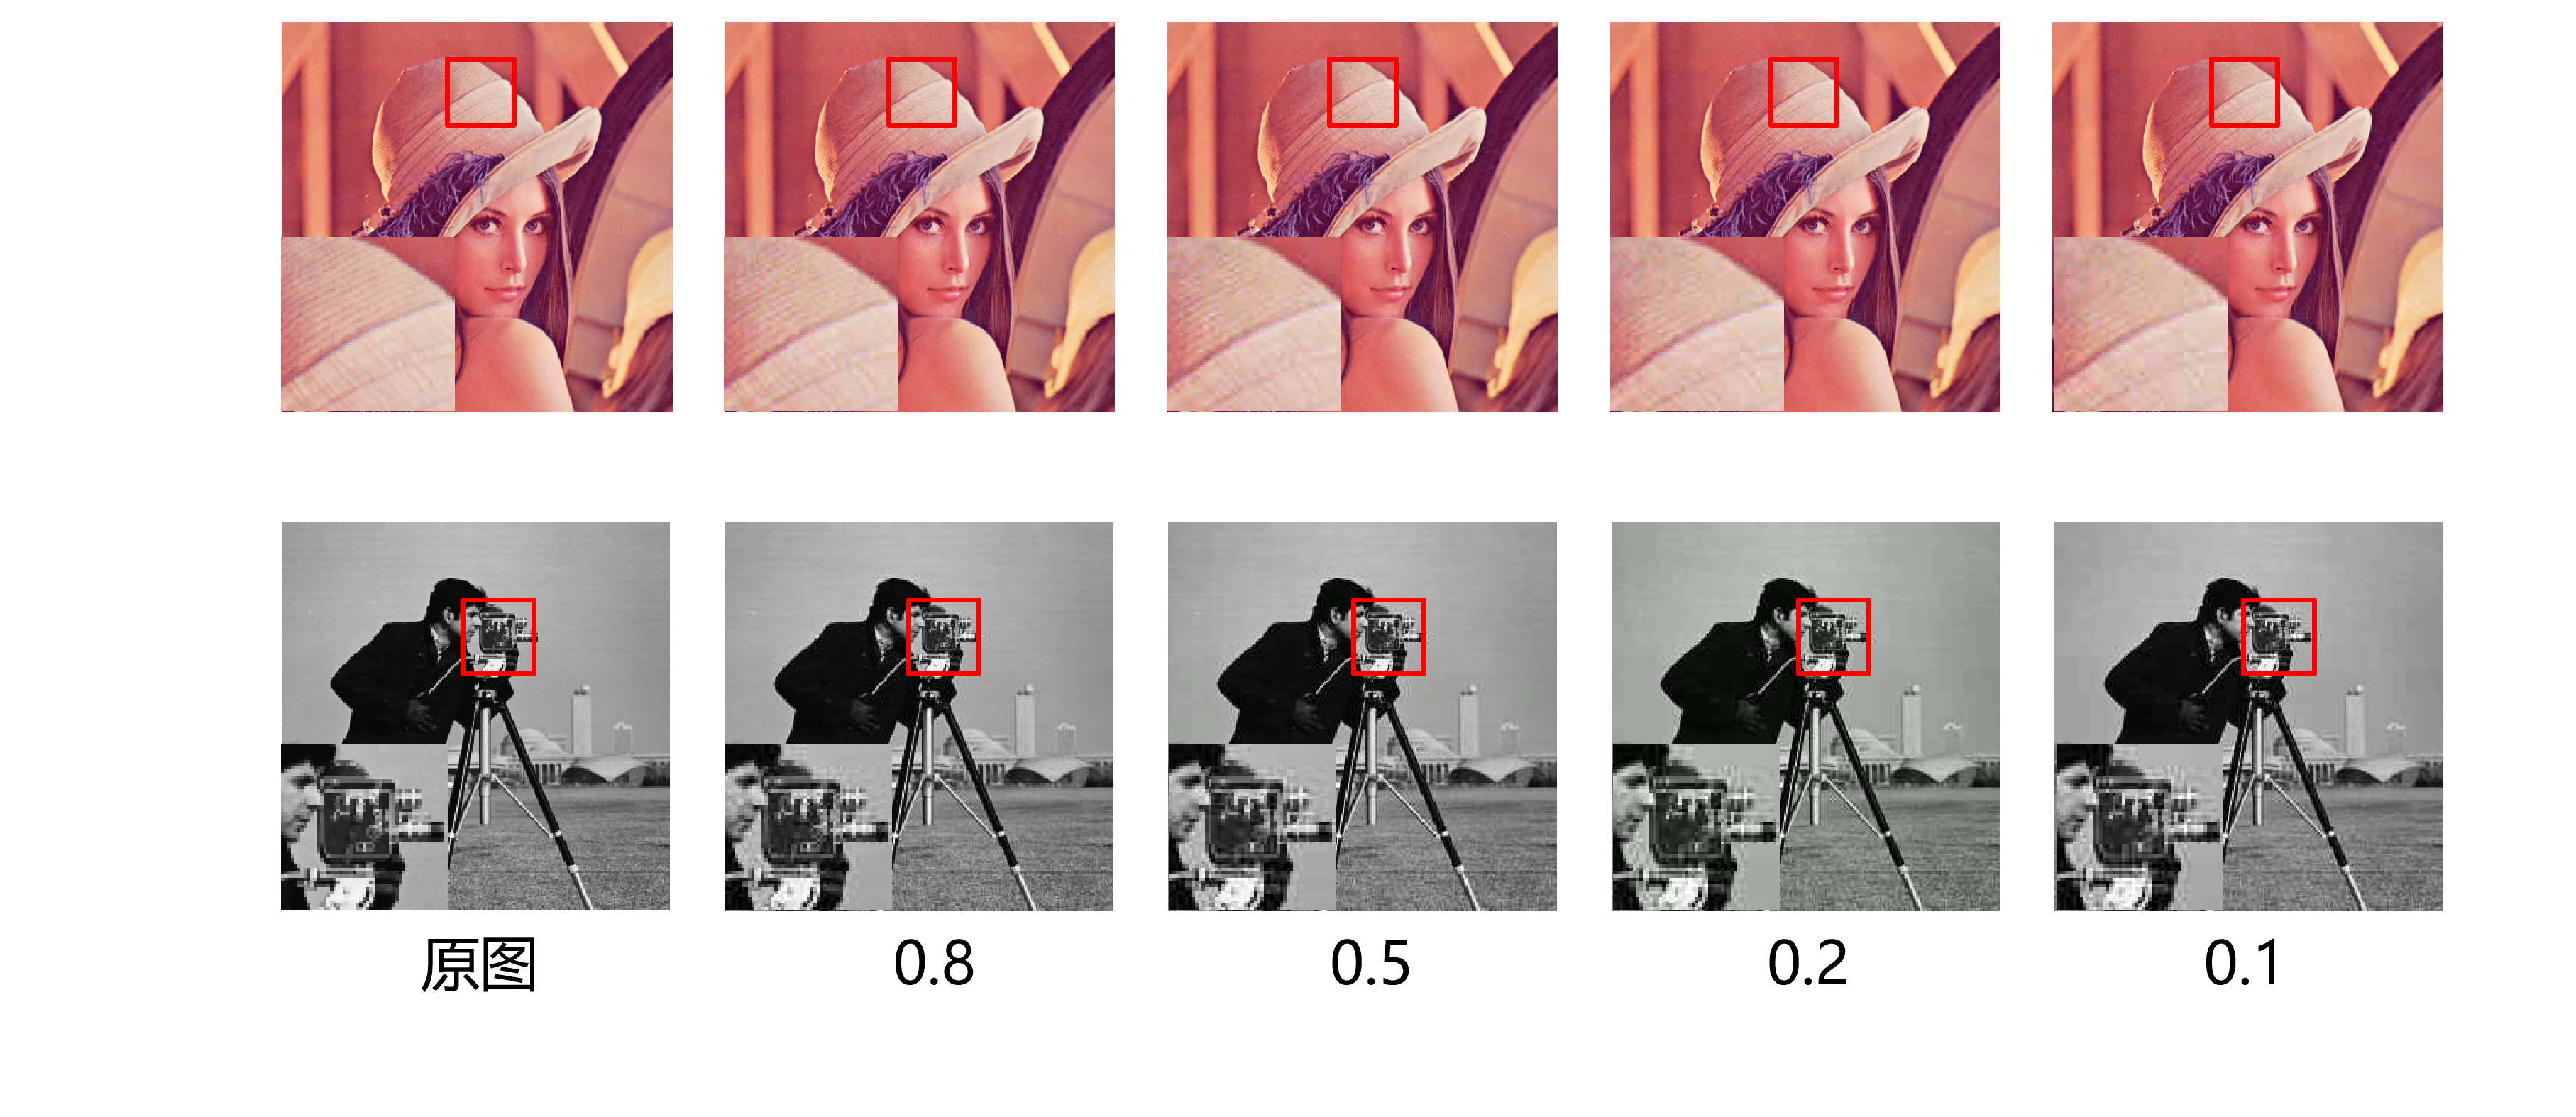
\includegraphics[width=1.0\textwidth]{pages/evaluation/result-image.png}
    \caption{实验结果的定性分析}
    \label{Fig.result}
\end{figure}

\section{实验结果的定量分析}
\subsection{性能指标}

\subsubsection{MSE}
均方误差(MSE)定义为原图各像素$I(i,j)$与压缩后图像各像素$K(i,j)$差的平方和(式\ref{Eq.MSE})
\begin{equation}
    MSE=\frac{1}{mn} \sum_{i=0}^{m-1}\sum_{j=0}^{n-1} [I(i,j)-K(i,j)]^2
    \label{Eq.MSE}
\end{equation}

\subsubsection{PSNR}
峰值信噪(PSNR)比定义为
\begin{equation}
    PSNR=20\lg (\frac{Max_1}{\sqrt{MSE}})
    \label{Eq.PSNR}
\end{equation}
其中$Max_1$是表示图像点颜色的最大数值,$MSE$为均方误差。


\subsubsection{SSIM}
样本$(x,y)$的结构相似度为
\begin{equation}
    SSIM(x,y)=\frac{2\mu_x\mu_y+C_1}{\mu_x^2+\mu_y^2+C_1}\cdot\frac{2\delta_{xy}+C_2}{\delta_x^2+\delta_y^2+C_2}
    \label{Eq.SSIM}
\end{equation}

\subsubsection{压缩比}

压缩比定义为原图片比特数与压缩后图片比特数之比。



\subsection{定量结果}

\begin{table}[h!]
    \begin{center}
        \caption{MSE}
        \begin{tabular}{c|ccccc}
            \textbf{压缩质量} & 0.8 & 0.5 & 0.3 & 0.2 & 0.1 \\
            \hline
            \textbf{MSE} & 4.92 & 5.40 & 5.73 & 5.90 & 6.00 \\
        \end{tabular}
    \end{center}
\end{table}


\begin{table}[h!]
    \begin{center}
        \caption{PSNR}
        \begin{tabular}{c|ccccc}
            \textbf{压缩质量} & 0.8 & 0.5 & 0.3 & 0.2 & 0.1 \\
            \hline
            \textbf{PSNR} & 41.2 & 40.8 & 40.5 & 40.4 & 40.3 \\
        \end{tabular}
    \end{center}
\end{table}

\begin{table}[h!]
    \begin{center}
        \caption{SSIM}
        \begin{tabular}{c|ccccc}
            \textbf{压缩质量} & 0.8 & 0.5 & 0.3 & 0.2 & 0.1 \\
            \hline
            \textbf{PSNR} & 0.98 & 0.98 & 0.98 & 0.98 & 0.98 \\
        \end{tabular}
    \end{center}
\end{table}



\begin{table}[h!]
    \begin{center}
        \caption{压缩比}
        \begin{tabular}{c|ccccc}
            \textbf{压缩质量} & 0.8 & 0.5 & 0.3 & 0.2 & 0.1 \\
            \hline
            \textbf{游程压缩比}     & 7.99 & 9.88 & 10.9 & 11.4 & 11.8 \\
            \textbf{总压缩比}       & 13.0 & 16.2 & 18.2 & 19.2 & 20.0 \\
            \textbf{Matlab压缩比}   & 17.8 & 32.3 & 44.5 & 56.6 & 82.2 \\
        \end{tabular}
    \end{center}
\end{table}
\end{document}
\chapter{图像有损压缩实验结果}

\section{实验结果的定性分析}
\begin{figure}
    \centering
    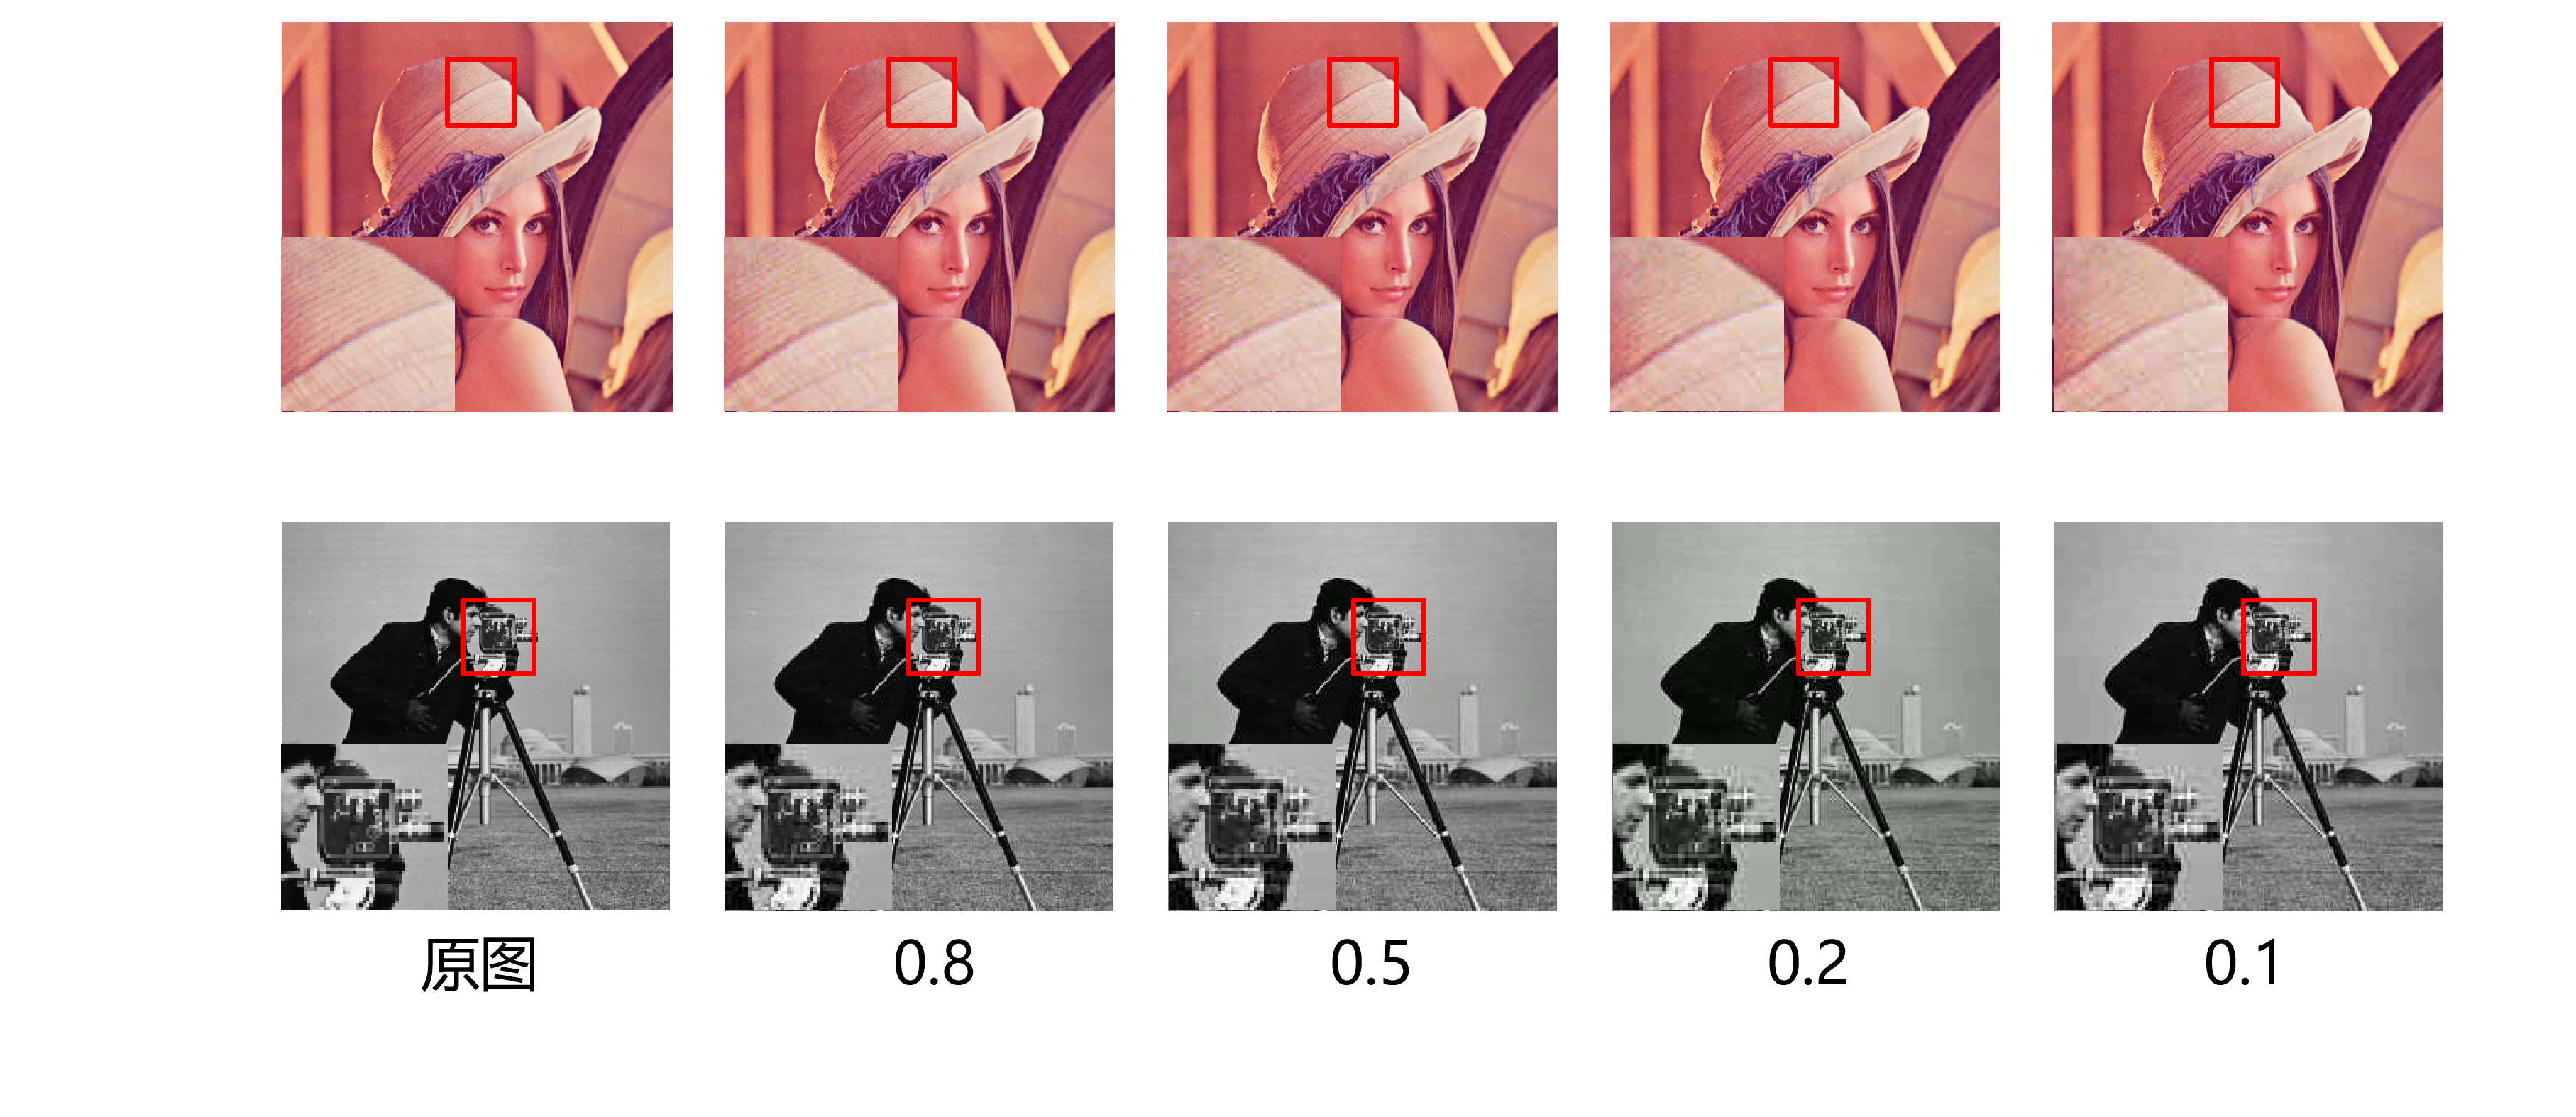
\includegraphics[width=1.0\textwidth]{pages/evaluation/result-image.png}
    \caption{实验结果的定性分析}
    \label{Fig.result}
\end{figure}

\section{实验结果的定量分析}
\subsection{性能指标}

\subsubsection{MSE}
均方误差(MSE)定义为原图各像素$I(i,j)$与压缩后图像各像素$K(i,j)$差的平方和(式\ref{Eq.MSE})
\begin{equation}
    MSE=\frac{1}{mn} \sum_{i=0}^{m-1}\sum_{j=0}^{n-1} [I(i,j)-K(i,j)]^2
    \label{Eq.MSE}
\end{equation}

\subsubsection{PSNR}
峰值信噪(PSNR)比定义为
\begin{equation}
    PSNR=20\lg (\frac{Max_1}{\sqrt{MSE}})
    \label{Eq.PSNR}
\end{equation}
其中$Max_1$是表示图像点颜色的最大数值,$MSE$为均方误差。


\subsubsection{SSIM}
样本$(x,y)$的结构相似度为
\begin{equation}
    SSIM(x,y)=\frac{2\mu_x\mu_y+C_1}{\mu_x^2+\mu_y^2+C_1}\cdot\frac{2\delta_{xy}+C_2}{\delta_x^2+\delta_y^2+C_2}
    \label{Eq.SSIM}
\end{equation}

\subsubsection{压缩比}

压缩比定义为原图片比特数与压缩后图片比特数之比。



\subsection{定量结果}

\begin{table}[h!]
    \begin{center}
        \caption{MSE}
        \begin{tabular}{c|ccccc}
            \textbf{压缩质量} & 0.8 & 0.5 & 0.3 & 0.2 & 0.1 \\
            \hline
            \textbf{MSE} & 4.92 & 5.40 & 5.73 & 5.90 & 6.00 \\
        \end{tabular}
    \end{center}
\end{table}


\begin{table}[h!]
    \begin{center}
        \caption{PSNR}
        \begin{tabular}{c|ccccc}
            \textbf{压缩质量} & 0.8 & 0.5 & 0.3 & 0.2 & 0.1 \\
            \hline
            \textbf{PSNR} & 41.2 & 40.8 & 40.5 & 40.4 & 40.3 \\
        \end{tabular}
    \end{center}
\end{table}

\begin{table}[h!]
    \begin{center}
        \caption{SSIM}
        \begin{tabular}{c|ccccc}
            \textbf{压缩质量} & 0.8 & 0.5 & 0.3 & 0.2 & 0.1 \\
            \hline
            \textbf{PSNR} & 0.98 & 0.98 & 0.98 & 0.98 & 0.98 \\
        \end{tabular}
    \end{center}
\end{table}



\begin{table}[h!]
    \begin{center}
        \caption{压缩比}
        \begin{tabular}{c|ccccc}
            \textbf{压缩质量} & 0.8 & 0.5 & 0.3 & 0.2 & 0.1 \\
            \hline
            \textbf{游程压缩比}     & 7.99 & 9.88 & 10.9 & 11.4 & 11.8 \\
            \textbf{总压缩比}       & 13.0 & 16.2 & 18.2 & 19.2 & 20.0 \\
            \textbf{Matlab压缩比}   & 17.8 & 32.3 & 44.5 & 56.6 & 82.2 \\
        \end{tabular}
    \end{center}
\end{table}
\end{document}
\chapter{图像有损压缩实验结果}

\section{实验结果的定性分析}
\begin{figure}
    \centering
    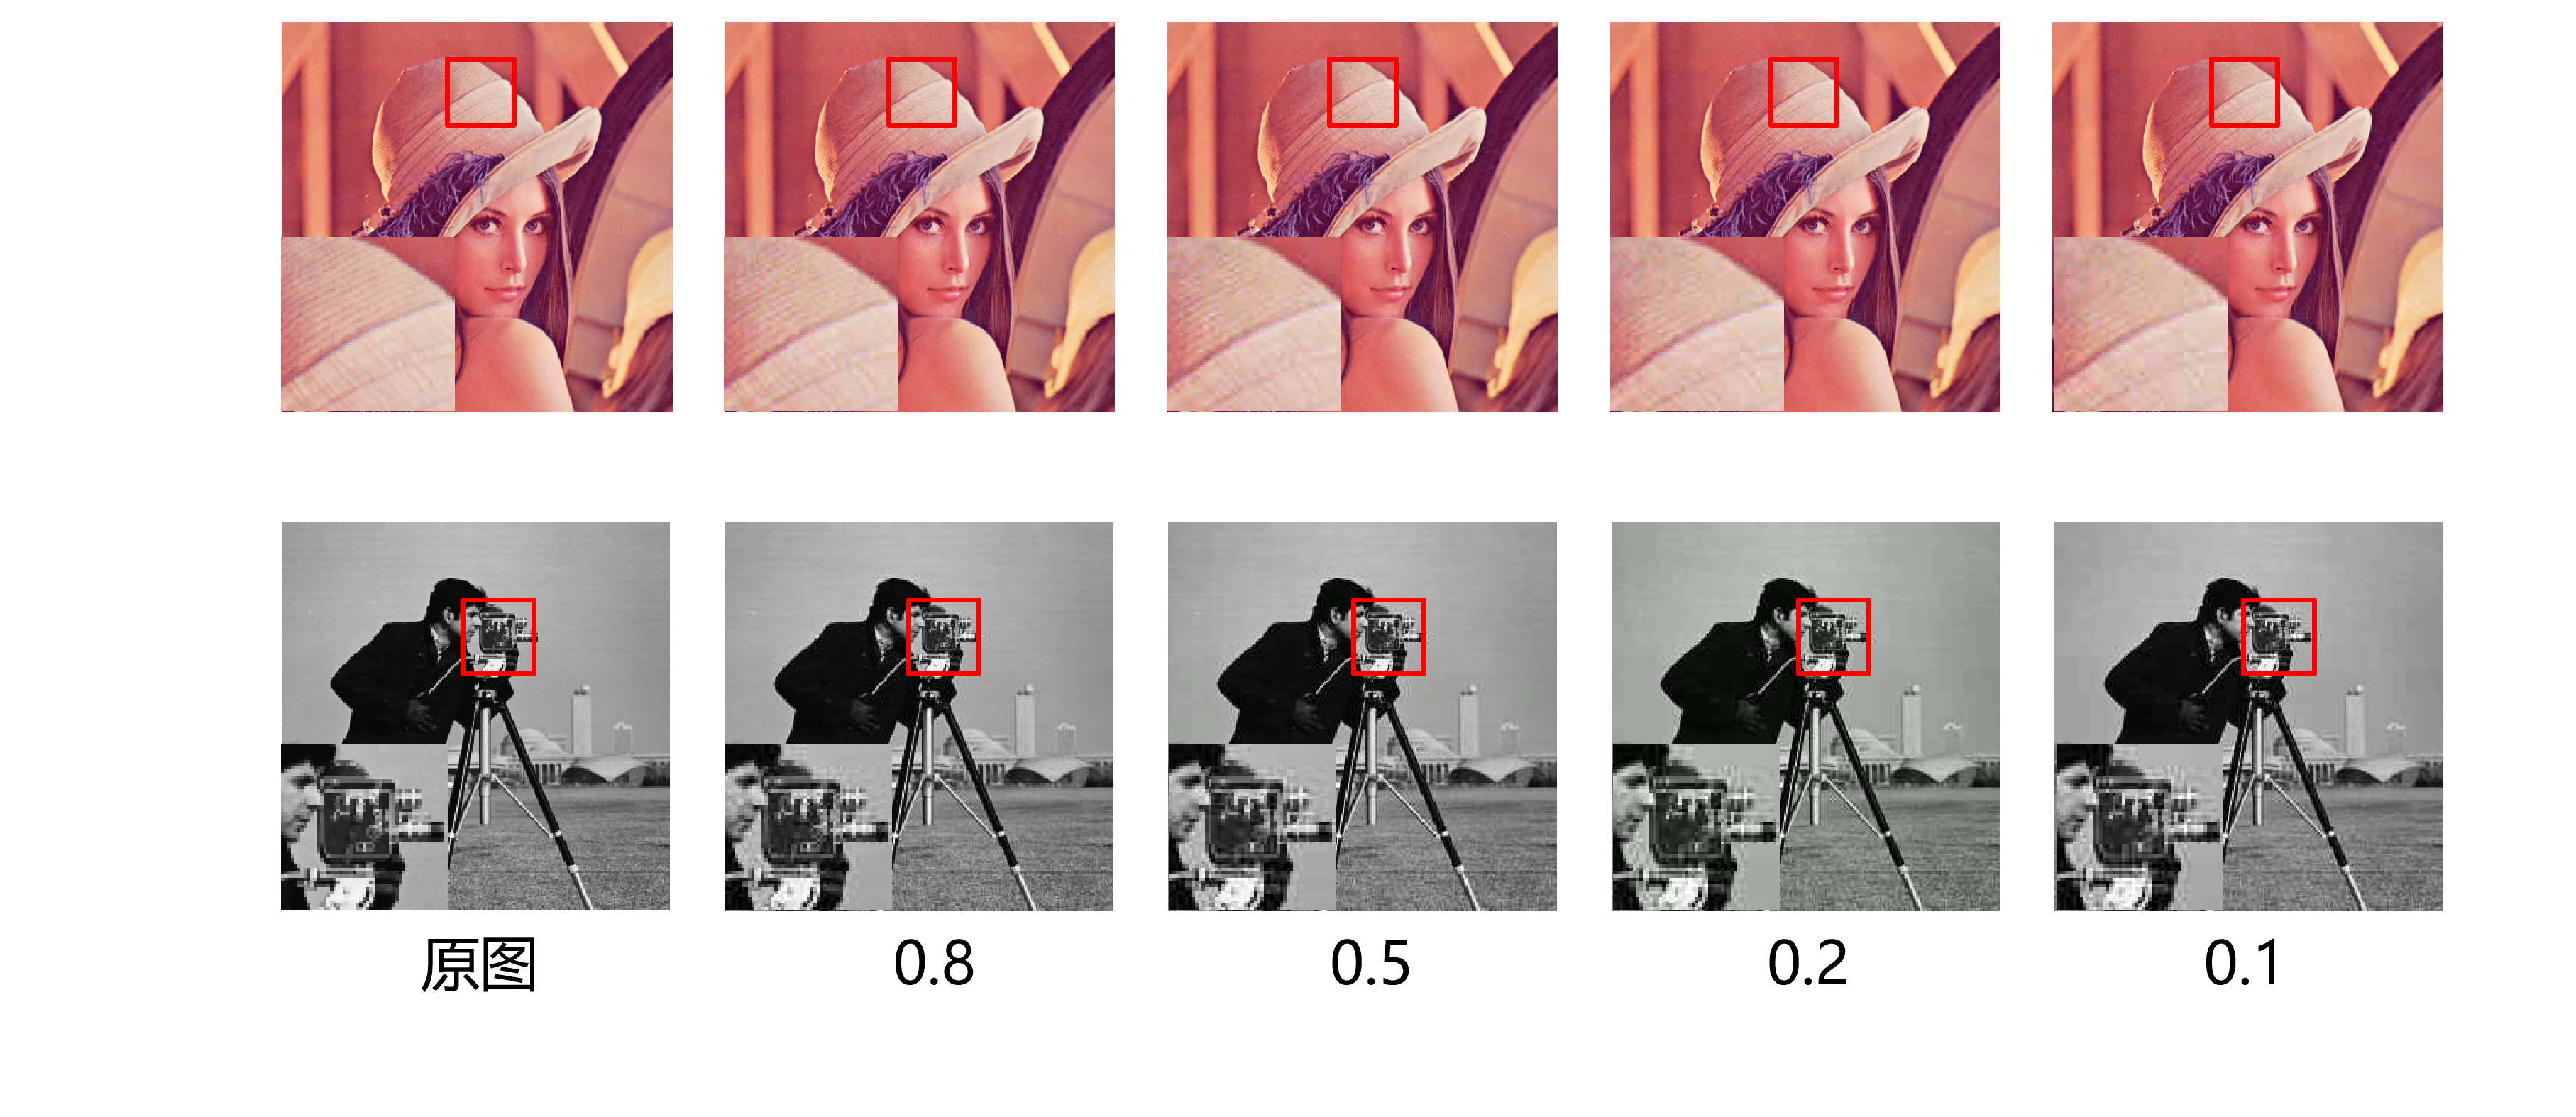
\includegraphics[width=1.0\textwidth]{pages/evaluation/result-image.png}
    \caption{实验结果的定性分析}
    \label{Fig.result}
\end{figure}

\section{实验结果的定量分析}
\subsection{性能指标}

\subsubsection{MSE}
均方误差(MSE)定义为原图各像素$I(i,j)$与压缩后图像各像素$K(i,j)$差的平方和(式\ref{Eq.MSE})
\begin{equation}
    MSE=\frac{1}{mn} \sum_{i=0}^{m-1}\sum_{j=0}^{n-1} [I(i,j)-K(i,j)]^2
    \label{Eq.MSE}
\end{equation}

\subsubsection{PSNR}
峰值信噪(PSNR)比定义为
\begin{equation}
    PSNR=20\lg (\frac{Max_1}{\sqrt{MSE}})
    \label{Eq.PSNR}
\end{equation}
其中$Max_1$是表示图像点颜色的最大数值,$MSE$为均方误差。


\subsubsection{SSIM}
样本$(x,y)$的结构相似度为
\begin{equation}
    SSIM(x,y)=\frac{2\mu_x\mu_y+C_1}{\mu_x^2+\mu_y^2+C_1}\cdot\frac{2\delta_{xy}+C_2}{\delta_x^2+\delta_y^2+C_2}
    \label{Eq.SSIM}
\end{equation}

\subsubsection{压缩比}

压缩比定义为原图片比特数与压缩后图片比特数之比。



\subsection{定量结果}

\begin{table}[h!]
    \begin{center}
        \caption{MSE}
        \begin{tabular}{c|ccccc}
            \textbf{压缩质量} & 0.8 & 0.5 & 0.3 & 0.2 & 0.1 \\
            \hline
            \textbf{MSE} & 4.92 & 5.40 & 5.73 & 5.90 & 6.00 \\
        \end{tabular}
    \end{center}
\end{table}


\begin{table}[h!]
    \begin{center}
        \caption{PSNR}
        \begin{tabular}{c|ccccc}
            \textbf{压缩质量} & 0.8 & 0.5 & 0.3 & 0.2 & 0.1 \\
            \hline
            \textbf{PSNR} & 41.2 & 40.8 & 40.5 & 40.4 & 40.3 \\
        \end{tabular}
    \end{center}
\end{table}

\begin{table}[h!]
    \begin{center}
        \caption{SSIM}
        \begin{tabular}{c|ccccc}
            \textbf{压缩质量} & 0.8 & 0.5 & 0.3 & 0.2 & 0.1 \\
            \hline
            \textbf{PSNR} & 0.98 & 0.98 & 0.98 & 0.98 & 0.98 \\
        \end{tabular}
    \end{center}
\end{table}



\begin{table}[h!]
    \begin{center}
        \caption{压缩比}
        \begin{tabular}{c|ccccc}
            \textbf{压缩质量} & 0.8 & 0.5 & 0.3 & 0.2 & 0.1 \\
            \hline
            \textbf{游程压缩比}     & 7.99 & 9.88 & 10.9 & 11.4 & 11.8 \\
            \textbf{总压缩比}       & 13.0 & 16.2 & 18.2 & 19.2 & 20.0 \\
            \textbf{Matlab压缩比}   & 17.8 & 32.3 & 44.5 & 56.6 & 82.2 \\
        \end{tabular}
    \end{center}
\end{table}
\end{document}